\documentclass[sigconf]{acmart}

\usepackage{booktabs} % For formal tables
\usepackage{amsmath,amssymb}
% \usepackage{cite}   % importing cite is throwing errors for some reason
\usepackage{color}
\usepackage{enumerate}
\usepackage{multicol}
\usepackage{float}

% \usepackage{tikz}
% \tikzset{
%   treenode/.style = {shape=rectangle, rounded corners,
%                      draw, align=center,
%                      top color=white, bottom color=blue!20},
%   root/.style     = {treenode, font=\Large, bottom color=red!30},
%   env/.style      = {treenode, font=\ttfamily\normalsize},
%   leaf/.style     = {treenode, font=\small, bottom color=green!30},
%   dummy/.style    = {circle,draw}
% }

% \usepackage{tikz-qtree}
% \usepackage{tikz-qtree-compat}
% \usetikzlibrary{positioning}
\usepackage{ textcomp }

% Get todos to render properly
\usepackage[obeyFinal]{easy-todo}

% Add package for well rendered quotations
\usepackage{dirtytalk}
\usepackage{hyperref}
\usepackage{graphicx}

\usepackage{lambda}

% correct bad hyphenation here
\hyphenation{op-tical net-works semi-conduc-tor}

% macro for angled brackets
\newcommand{\brackets}[1]{$\langle$\ignorespaces#1\unskip$\rangle$}
% Copyright
%\setcopyright{none}
%\setcopyright{acmcopyright}
%\setcopyright{acmlicensed}
\setcopyright{rightsretained}
%\setcopyright{usgov}
%\setcopyright{usgovmixed}
%\setcopyright{cagov}
%\setcopyright{cagovmixed}


% DOI
\acmDOI{10.475/123_4}

% ISBN
\acmISBN{123-4567-24-567/08/06}

%Conference
\acmConference[Seattle'2017]{SIGCSE}{March 2017}{Seattle, Washington USA} 
\acmYear{2017}
\copyrightyear{2017}

\acmPrice{15.00}


\begin{document}
\title{A Domain Analysis of Data Structure and Algorithm Explanations in the Wild}


% \author{Jeffrey Young} 
% \affiliation{%
%  \institution{Oregon State University}
%  \department{School of EECS}
%  \city{Corvallis} 
%  \state{Oregon}
%  \country{USA}}
% \author{Eric Walkingshaw} 
% \affiliation{%
%  \institution{Oregon State University}
%  \department{School of EECS}
%  \city{Corvallis} 
%  \state{Oregon}
%  \country{USA}}
\author{Anonymized for Review}


\begin{abstract}
  Explanations of data structures and algorithms are complex interactions of
  several notations, including natural language, mathematics, pseudocode, and
  diagrams. Currently, such explanations are created ad hoc using a variety of
  tools, and the resulting artifacts are static, reducing explanatory value. We
  envision a domain-specific language for developing rich, interactive
  explanations of data structures and algorithms. In this paper, we analyze this
  domain to sketch requirements for our language. We perform a grounded theory
  analysis, to generate a qualitative coding system for explanation artifacts
  collected online. We show that grounded theory provides a robust methodology
  for analyzing qualitative objects and that the resultant coding system forms
  the skeleton of a domain-specific language. This work is part of our effort to
  develop the paradigm of explanation-oriented programming, which shifts the
  focus of programming from computing results to producing rich explanations of
  how those results were computed.
\end{abstract}

%
% The code below should be generated by the tool at
% http://dl.acm.org/ccs.cfm
% Please copy and paste the code instead of the example below. 
%
% \begin{CCSXML}
% <ccs2012>
%  <concept>
%   <concept_id>10010520.10010553.10010562</concept_id>
%   <concept_desc>Computer systems organization~Embedded systems</concept_desc>
%   <concept_significance>500</concept_significance>
%  </concept>
%  <concept>
%   <concept_id>10010520.10010575.10010755</concept_id>
%   <concept_desc>Computer systems organization~Redundancy</concept_desc>
%   <concept_significance>300</concept_significance>
%  </concept>
%  <concept>
%   <concept_id>10010520.10010553.10010554</concept_id>
%   <concept_desc>Computer systems organization~Robotics</concept_desc>
%   <concept_significance>100</concept_significance>
%  </concept>
%  <concept>
%   <concept_id>10003033.10003083.10003095</concept_id>
%   <concept_desc>Networks~Network reliability</concept_desc>
%   <concept_significance>100</concept_significance>
%  </concept>
% </ccs2012>  
% \end{CCSXML}

% \ccsdesc[500]{Computer systems organization~Embedded systems}
% \ccsdesc[300]{Computer systems organization~Redundancy}
% \ccsdesc{Computer systems organization~Robotics}
% \ccsdesc[100]{Networks~Network reliability}


% \keywords{ACM proceedings, \LaTeX, text tagging}

\maketitle

\section{Introduction}
\label{sec:intro}

Data structures and algorithms are at the heart of computer science and must be
explained to each new generation of students. A pressing question is: How can we
do this effectively?

In this paper, we focus on the \emph{artifacts} that constitute or support
explanations of data structures and algorithms (hereafter just ``algorithms''),
which can be shared and reused.
%
For verbal explanations, such as a lecture, the supporting artifact might be
the associated slides. For written explanations, the artifact is the
explanation as a whole, including the text and any supporting figures.
%
Explanation artifacts associated with algorithms are interesting because they
typically present a complex interaction among many different notations,
including natural language, mathematics, pseudocode, executable code, various
kinds of diagrams, animations, and more.


Currently, explanation artifacts for algorithms are created ad hoc using a
variety of tools and techniques, and the resulting explanations tend to be
static, reducing their explanatory value.
%
Although there has been a substantial amount of work on algorithm visualization~
\cite{Gloor92,Gloor97,HDS02, shaffer2010algorithm, HANSEN2002291, KANN1997223},
and tools exist for creating these kinds of supporting artifacts, there is no
good solution for creating integrated, multi-notational explanations as a whole.
Similarly, although some algorithm visualization tools provide a means for the
student to tweak the parameters or inputs to an algorithm to generate new
visualizations, they do not support creating cohesive interactive explanations
that correspondingly modify the surrounding explanation or that allow the
student to respond to or query the explanation in other ways.
%
To fill this gap, we envision a \emph{domain-specific language} (DSL) that
supports the creation of rich, interactive, multi-notational artifacts for
explaining algorithms.
%
The development of this DSL is part of a larger effort to explore the new
paradigm of \emph{explanation-oriented programming}, briefly described in
Section~ \ref{sec:back:xop}.


The intended users of the envisioned DSL are CS educators who want to create
\emph{interactive artifacts} to support the explanation of algorithms. These
users are experts on the corresponding algorithms, and also trained and skilled
programmers. The produced explanation artifacts might supplement a lecture or
be posted to a web page as a self-contained (textual and graphical)
explanation.
%
The DSL should support pedagogical methods directly through built-in
abstractions and language constructs. It should also support a variety of forms
of student interaction. For example, teachers should be able to define
equivalence relations enabling users to automatically generate variant
explanations~\cite{EW13jvlc}, to build in specific responses to anticipated
questions, and to provide explanations at multiple levels of abstraction.


This paper represents a formative step toward this vision. We conduct a
\emph{qualitative analysis} of our domain in order to determine the form and
content of the explanation artifacts that educators are already creating.
%
We base our analysis on an established qualitative research method called
\emph{grounded theory}~\cite{Strauss67discoveryof} in order to better understand how well existing artifacts
explain complex topics


More specifically, we collect 15 explanation artifacts from the internet,
consisting of only lecture notes that explain two algorithms and one
data structure commonly covered in undergraduate computer science courses:
Dijkstra's shortest path algorithm~\cite[pp.~137--142]{KT06}, merge sort
~\cite[210--214]{KT06}, and AVL trees~\cite[pp.~458--475]{KnuthArt3}.
%
We analyze these artifacts through the application of grounded
theory~\cite{Strauss67discoveryof}, a formal method for analyzing qualitative
data that originated in sociological research. Through the application of
grounded theory, we develop a coding system that captures the structure of
explanation for each document. An overview of the coding system is given in
Section \ref{sec:res:sys}.

% We analyze these artifacts by applying a classic pedagogical theory by Bellack
% et al.~\cite{bellack1966language} that describes the patterns of language used
% in the process of teaching. Bellack et al.\ define a typology for coding
% transcripts of teacher and student verbalizations during teaching. An overview
% of the typology is given in Section~\ref{sec:back:typ}.


This paper makes the following contributions:
%
\begin{enumerate}[C1.]

\item \label{contrib:method}
  We provide a case study on analyzing \emph{qualitative data} through the
  application of a formal research method \emph{grounded theory}, that is not
  part of the computer science parlance.

\item \label{contrib:data}
%
We provide a coded qualitative data set of explanation artifacts, using the
system defined in C\ref{contrib:codes} applied to our sample of 15 collected
explanation artifacts (Section~\ref{sec:exp:data}).

\item \label{contrib:codes}
%
\todo{decide if we need to split this contribution up}
We provide a coding system for analyzing \emph{explanation artifacts} in the
form of lecture notes, and we show that through the application of the coding
system, each such artifact forms a tree structure, which we have termed a
\emph{explanation tree}

\todo{tie this in} One of the central dilemmas of analyzing explanations in the
wild is that they vary widely and do not directly map onto any perceivable
shared, abstract structure. If explanation-oriented programming is to become a
viable paradigm then this formative problem must be solved. A major step forward
in this direction is the concept of \emph{explanation trees}. In this paper, use
a coding system grounded in the data to observe a shared structure between
explanations of like content and dissimilar content, lengths, authors, and
institutions. We believe that such a structure forms the building blocks of
\todo{something}

(Section \ref{sec:res:xopTree}).


\item \label{contrib:DSL}
%
  We describe how a coding system grounded in data can provide a
  semantics basis for a DSL and argue for the advantages of such an approach
  (Section~\ref{sec:res:DSL}).
%
\end{enumerate}

\noindent

\section{Background And Related Works}
\label{sec:back}

\todo{Add related works to this section, get some sources}
In this section, we put the present work into context by the describing the
paradigm of \emph{explanation-oriented programming} in
Section~\ref{sec:back:xop}, the exploration of which is an underlying
motivation of our work, and by introducing the methodology of grounded theory
~\cite{Strauss67discoveryof} in Section~\ref{sec:back:gt}, which is the
theoretical foundation of our coding system.

\subsection{Explanation-oriented programming}
\label{sec:back:xop}

\emph{Explanation-oriented programming} (XOP) is a new programming paradigm
% originally proposed at VL/HCC~2008~\cite{EW08vl},
where the primary output of a program is not a set of computed values, but an
\emph{explanation of how} those values were
computed~\cite{EW08vl,EW09dsl,EW09vl,WE11dsl,EW13jvlc}.
%
A high-level goal of this work is to further develop the paradigm of XOP
through the development of a specific DSL.


Programming languages for XOP should not merely produce explanations as a
byproduct, but should provide abstractions and features specific to the
creation of interactive explanation artifacts. For example, they should provide
facilities for creating application-specific notations and visualizations
(which are widespread in explanations of algorithms), and for describing
alternative explanations produced in response to user input, for example, at
different levels of abstraction, by parameterization, or generated by
explanation equivalence laws~\cite{EW13jvlc}. Additionally, languages for XOP
should help guide the programmer toward the creation of \emph{good}
explanations.


The need for interactive explanation artifacts is motivated by the observation
that there is a trade-off between personal explanations and traditional
explanation artifacts, which can be partially bridged by XOP programs viewed as
rich, interactive explanation artifacts.
%
A good \emph{personal explanation} is useful because the explainer can
\emph{respond} to the student, adjusting the pace and strategy as necessary.
For example, the teacher can answer questions, rephrase parts of an
explanation, and provide additional examples as needed.
%
Unfortunately, good personal explanations are a scarce resource. First, there
are limited number of people who can provide high quality personal explanations
on a topic. Second, a personal explanation is usually ephemeral and so cannot
be directly shared or reused.
%
Since personal explanations are hard to come by, many students learn from
\emph{impersonal explanation artifacts}, such as recorded lectures, textbooks
and online written and graphical resources.
%
These impersonal explanations lack the interaction and adaptability of personal
explanations, but have the advantage of being easy to massively share and reuse
via libraries and the internet.


In-person lectures, such as those covering algorithms in most undergraduate
computer science programs, exist at a midway point between impersonal and
personal explanations, perhaps closer to the personal end of the spectrum.
These \emph{classroom explanations} are adaptable---students can ask questions
in class, the teacher can respond, and explanations can be adapted on the fly
if students are confused---but they are not as adaptable as personal
explanations since the teacher must accommodate many students at once.
Classroom explanations are more efficient than personal explanations since they
are shared amongst many students, but not as efficient as impersonal
explanations since they are still ephemeral and therefore difficult to reuse.


We target another midway point, a bit closer to the impersonal end of the
spectrum, of \emph{interactive explanation artifacts} that provide as much of
the responsiveness and adaptability of personal explanations as possible, but
which can still be massively shared and reused online. Such an explanation
artifact would be quite expensive to produce with current tools since an
\emph{explanation designer} must not only construct a high quality initial
explanation and corresponding visualizations, but also anticipate and
explicitly program in responses to queries by the student.
%
We expect that DSLs for XOP can help alleviate this burden.


% To help realize this vision, our medium-term goal is to design a
% \emph{domain-specific language} (DSL) that supports the creation of interactive
% explanation artifacts. This DSL is part of our larger effort to explore the
% paradigm of \emph{explanation-oriented programming}


% As a step in this development, we aim to design and implement a domain-specific
% language (DSL) in the XOP paradigm to support computer science education. 

\subsection{Grounded Theory}
\label{sec:back:gt}
In this section we present an overview of the research method known as grounded
theory. This section is meant to help orient the reader to understand the
process by which the coding system was formed.

%% What is it
The central idea behind grounded theory is to generate, or discover theory,
inductively, \emph{based on data} rather than to use data to evince a hypothesis
of a theory. Grounded theory is rooted in a \emph{pragmatist} view of theory
i.e. that theory should be purposed and suited towards its intended uses
vis-a-viz logico-deductive theories which are concerned with what can be
expressed by the theory~\cite{Strauss67discoveryof}. As Glaser and Strauss
state:
\newline
\newline
\say{A grounded theory is one that is inductively derived from the study of
the phenomena it represents}.
\newline
\newline
Like any methodology, grounded theory employs a specific vocabulary to refer to
stages and phases of research. The rest of this section will introduce grounded theory
terminology in concert with an operational example that will show how one may
actually perform a grounded theory analysis.


Imagine a researcher who wants to find out why students drop out of
Computer Science programs. The first task for a grounded theorist would be to
collect data from the subject they wish to study. This data would most likely be
in the form of interviews with the students, their schedule, and example
homework assignments. Once some data is collected the research will begin
\emph{coding}, coding is the act of taking qualitative data e.g lecture notes,
an interview, personal letters and assigning tags that describes the data.
 
Coding consists of three stages~\cite{corbin2014basics}: First, a researcher
performs \emph{open coding}. In open coding, one writes down \emph{any} term or
terms that describes the data, regardless of duplicate or related concepts. In
our example these tags could be things such as the year of a student, nicknames
that people call one another, things about their life, family, or activities.
Open coding should make use of \emph{in vivo} terms, these are terms that people
immersed in the culture use. For example, a computer scientist may discuss the
``recurrence relation'', while a factory worker may use the term ``floor boss''
to mean the manager.
 
The second stage of coding is called \emph{axial coding}, in axial coding the
researcher identifies the relationships between the tags developed in open
coding. The goal is to develop a \emph{coding paradigm}, which is a model that
displays the inter-relationship between codes~\cite{corbin2014basics}. An axial
code for our example may coalesce sets of open codes to several axial codes. For
example, if one had the open codes ``tired, exhausted, no time for other
activities, stressed from homework'', these might inform the axial code ``burn
out''.
 
\emph{selective coding} is the final stage of coding, in this stage the
researcher tries to identify a few central tags that form the basis for the
theory. After identifying these core tags the researcher then seeks to relate
the core tags to the remaining tags. In our example, we might have
the axial codes ``burn out, no support, everyone is perceived better, anxiety
over schoolwork'' and conclude that the selective code would be
``impostor syndrome''.
 
All phases of research proceed in parallel to data collection and analysis. That
is to say that the researcher in our example will be simultaneously collecting
data, coding, forming their theory, and moving between each activity at the
same time . This is a marked departure from quantitative methods where phases
are distinct and disjunct~\cite{Strauss67discoveryof}.


Through coding, the researcher interacts with their data. But how does that
researcher know when to stop coding? Or how much data to code? Such questions
are the motivation for three central tenets in grounded theory.
 
The first is called \emph{constant comparison}, the idea is that during coding,
the researcher must think back and ask if they are being consistent. Researchers
should perform this check constantly and at every stage of coding as it is
pivotal to the validity of the method~\cite{Strauss67discoveryof}.
 
The second tenet is \emph{theoretical sampling}; theoretical sampling, focuses
on filling the \emph{perceived} gaps in data based on current theory. To put
this into context, if the researcher in our example were a quantitative
researcher they would determine the total student population of the CS program,
and then use statistics to generate a representative data set. The grounded
theory researcher, would look at their data and determine that they do not have
any data points from people who have taken the operating systems class, thus
they will collect more data to fill that gap \emph{based on their current
  results}.
 
The last tenet describes how to reach an end point in coding; grounded theorists
call it \emph{saturation}. Saturation occurs when new data is added to the
researcher's data set and no new tags or modifications to the coding system are
required. This is when the researcher's system is able to express data that was
\emph{not} used to generate it. The requisite number of data to reach this point
may vary drastically based on factors such as researcher, topic, and motivating
research questions.


%% How it was used and Why
% For this study, saturation was reached at 11 documents.
% In this study, grounded theory was employed to generate a \emph{coding paradigm}
% about explanation artifacts. Our resultant theory is that explanation artifacts
% correspond to a pre-order traversal of an \emph{explanation tree}. Such trees,
% expressed in the coding system, distill the essence of a given explanation
% artifact. \todo{Eric's thoughts on flowery language}

\section{Experimental Setup}
\label{sec:exp:data}
In this section we describe how the data was collected, any preprocessing the
data may have undergone, and the system used to apply tags to the data. 

We restrict the scope of data collection to include only artifacts that provide
an explanation of common computer science algorithms from computer science
departments at accredited universities. Restricting the scope of artifacts in
this manner provides two benefits: 1) All explanatory artifacts have a stated,
intrinsic goal to communicate the mechanics, application, or implementation of
some common computer science algorithm. 2) There are bountiful and varied
examples of different approaches to explain \emph{the same} algorithm, and
numerous examples of \emph{like} approaches to explain different algorithms. All
data collected was either in PDF file format, or an html file that was converted
to PDF. No powerpoint lecture notes were considered because we feared that such
documents would be information scarce; powerpoints are used to structure a
lecture and thus should be considered with the concomitant lecture.

All data was coded by hand with the aid of Atlast.ti software~\cite{atlast} by a
single researcher. The use of the Atlast.ti software was primarily for
organizational and representational benefit, such as generating the code list
and performing constant comparison.
%
The use of such software is contingent with respect to grounded theory.
% This analysis, and any other grounded theory analysis, could be performed without such an aid.
%
If a document drifted substantially into a different algorithm then that section
was not considered. For example, if a document explaining Dijkstra's algorithm,
discussed shortest-path problems, then this was considered as it is directly
relevant to explaining Dijkstra's algorithm, but if that document included a
section on explaining Bellman-Ford's algorithm, then this section was not
considered as it's purpose is not to \emph{explain} Dijkstra's algorithm.

Explanatory artifacts were indexed according to the algorithm that was to be
explained, and a simple counter. For example, the first document regarding AVL
Trees would be named ``AVT01'' while the sixth would be ``AVT06'' and so on.
All of the data in this paper was collected and analyzed by a single researcher.

We made no attempt to restrict the size of the data collected, in order to
collect a diverse set of data. The smallest document collected has only a page
and a half of relevant material while the longest consists of eighteen pages.
All data can be found the projects github repository\footnote[1]{anonymized for
  review} Fifteen documents were coded in total, with five documents each per
algorithm.

Lastly, selective coding was not attempted or performed. The goal of this study
was to develop a prototype coding system, not to develop an overarching, causal
theory for these documents.

\section{Results}
In this section we present our findings. We make three major observations from
the data. First, we observe that the data is able to be expressed in the coding
system and provide an overview of the coding system in Section \ref{sec:res:sys}
and provide a sample coding. In Section \ref{sec:res:xopTree} we observe that
when data is expressed through the lens of the coding system, the result is an
explanation tree, and that the content of each document is expressed with a
pre-order traversal of the corresponding explanation tree.

\subsection{The Coding System}
\label{sec:res:sys}

The complete grammar is shown in table~\ref{res:tbl:grmr}.

\CatchFileDef{\TableHeader}{TableHeader.tex}{}
\CatchFileDef{\StructTable}{StructTable.tex}{}
\CatchFileDef{\AspectTable}{AspectTable.tex}{}
\CatchFileDef{\MoveTable}{MoveTable.tex}{}
\CatchFileDef{\DecoratorTable}{DecoratorTable.tex}{}
\begin{table*}
  \begin{tabular}{l p{1.8\linewidth}}

    \TableHeader
    \\
    % \StructTable
    % \\
    % \AspectTable
    % \\
    % \MoveTable
    % \\
    \DecoratorTable
    
  \end{tabular}
  \caption{Grammar for Coding System}
  \label{res:tbl:grmr}
\end{table*}


\begin{table}[H]
  \begin{tabular}{c p{0.8\linewidth} l}

    & Text & Coding \\
    \hline
    1 & \textbf{2.2 Mergesort} & Algorithm \\
    \\

    2 & The algorithms that we consider in this section is based on a simple operation
    known as merging: combining two ordered arrays to make one larger ordered
    array. & -> Operation Description InVivo\\
    \\

    3 & This operation immediately lends itself to a simple recursive sort
    method known as mergesort: to sort an array, divide it into two halves, sort
    the two halves (recursively), and then merge the results. & pop Description \\
    \\

    4 & \text{<cartoon of list>} & Cartoon \\
    \\

    5 & Mergesort guarantees to sort an array of N items in time proportional to N log
    N, no matter what the input. & -> Motivation Description \\
    \\

    6 & Its prime disadvantage is that it uses extra space proportional to N. & |
    Disadvantage Description \\
    \\

    7 & \textbf{Abstract in-place merge.} & | Operation
  \end{tabular}
  \caption{Sample text and codings for beginning of MS03, bolded text are headers}
  \label{res:txt:ex}
  \todo{fix location and formatting, ask eric what this should look like}
\end{table}
  
   

The coding system consists of 4 finite sets of tags. Context tags determine what
subject is being discussed in the corresponding section of the document.
%
Structuring tags construct and traverse the structure of the document. The
push and swap tags take a single context tag as input and creates a sub-context
for that input tag. For example in row 5 of example~\ref{res:txt:ex}, the
snippet exists in the context ``Algorithm'', thus ``push Motivation'' will
create a sub-context that denotes \emph{the motivation of the Algorithm}.
%
The pop tag takes any number of action and expression tags, lifts one level of
context, and then applies the input tags. Note that if a pop and push tags occur
in the same sequence, pop is always applied before push. The return tag takes no
input, and pops until reaching the root context. The swap tag takes a single
context tag as input, and any number of action or expression tags and then pops
out of a sub-context, creates a new sub-context with that input tag, and
then applies the non-content tags it is synonymous with the sequence ``pop push
<input tags>''.
%
When a context tag is \emph{orphaned} as in example~\ref{res:txt:ex}
\todo{reference rows in a table?}, then that is interpreted as returning to the
top level scope and then sub scoping into that tags context. The first tag in
every document is interpreted as setting the \emph{root} node of that particular
document. For instance, in example~\ref{res:txt:ex} row 1, the first tag:
``Algorithm'', sets the root context for the entire example.
%
Action tags determine what the document is \emph{doing} for a given section.
These tags are concrete things that are being done in the text, such as: Giving
an example, providing an outline, describing something, concluding a point, or
giving a proof. Action tags may occur alone or with any other tags. When action
tags are orphaned then this is interpreted as adding that action to the current
context. For example, rows 2, 3 and 4 in table~\ref{res:txt:ex}, occur in the
context ``Algorithm'', thus these are interpreted as: The document is discussing
an Algorithm; giving a description of it and introducing an in vivo term (row
2); 
%
Expression tags denote \emph{how} the context is being expressed in the current
context, some examples are: Cartoon, PseudoCode, Code, and Table. Expression
tags may be orphaned or occur with any other tag. Modifier tags alter the
semantic meaning of content tags that they are applied, each is a special case
described in table~\ref{res:tbl:grmr}.
%

\subsection{Explanation Trees}
\label{sec:res:xopTree}
The coding system borne out of the data is, in essence, one used to describe a
tree structure. This conclusion was born out of necessity during axial coding
and became the \emph{coding paradigm} for this study. The central problem was to
keep track of the different topics each document would discuss throughout their
duration. This led directly to the creation of content and structure tags, which
upon retrospection clearly formulate the document into a tree structure. An
example tree is given below for document, constructed, by hand, via
graphiz~\cite{Ellson2002}.

\begin{figure}[t]
  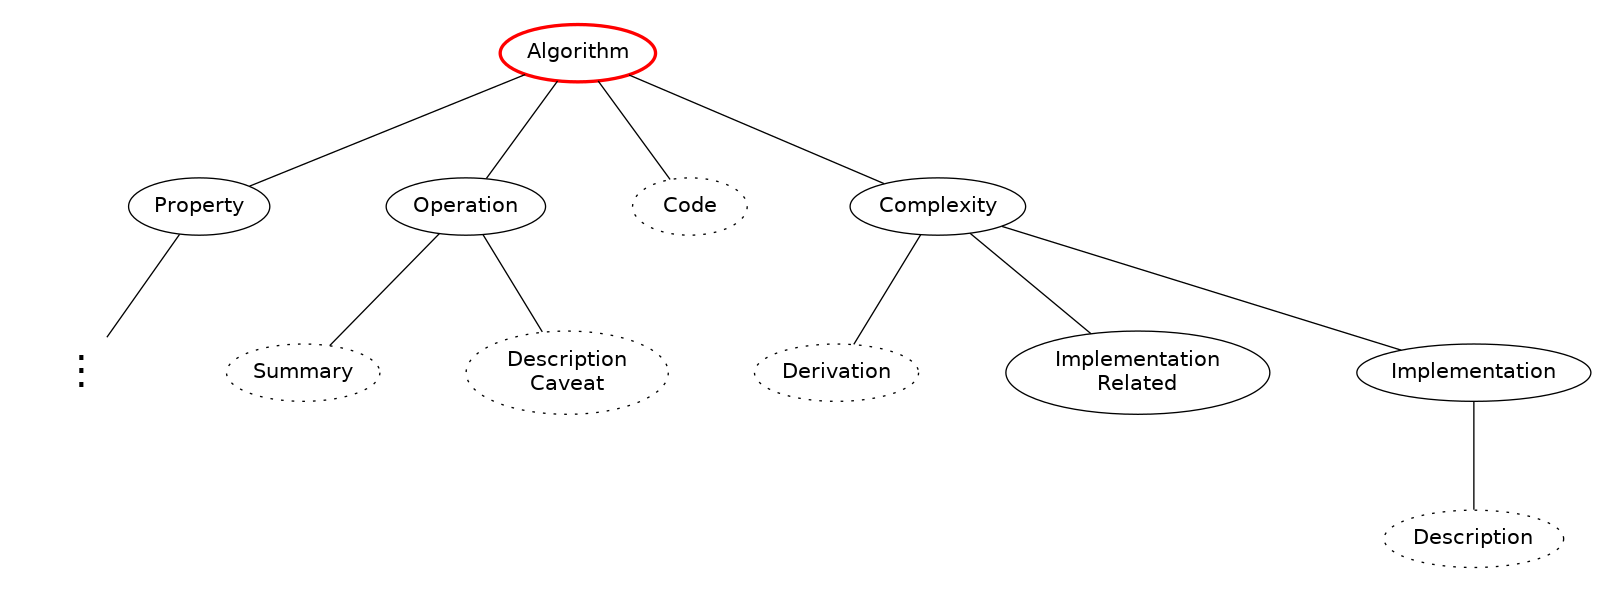
\includegraphics[scale=0.5, trim={0.2cm 0.5cm 0.5cm 0.5cm},clip]{DJK_tree}
\caption{Explanation Tree for Dijkstra's 04}
\label{fig:djk-tree}
\end{figure}

Figure~\ref{fig:djk-tree} displays the explanation tree of an explanation
artifact for Dijkstra's algorithm, that has been slightly altered to provide a
useful example. By observation, a pre-order traversal of this tree corresponds
with a normal reading of the document. Content tags become nodes in the
explanation tree, and the context is set by the path to a given node. For
example, if the context path is \brackets{Algorithm, Operation} then the context
is discussing the ``Operation'' of the ``Algorithm'', as seen in
figure~\ref{fig:djk-tree}. Actions as leaves in the tree. If the action occurs
in the code coincident with a structure and content tag, then it is represented
in the tree as leaf of the child context as seen in the ``Operation'' node. If
an action tag appears without a content tag, then it represents a terminal leaf
attached to the current node, as shown in the root node. If an action tag
appears coincident with the pop operator then it manifests as a leaf, on the
parent of the current node. This corresponds with popping the context, and then
applying the action. Expression tags are represented as terminal leaf nodes, as
seen at ``Code'' in figure~\ref{fig:djk-tree}. Modifier tags are represented as
labels that are attached to their input tags, regardless of how those input tags
manifest, some examples are nodes ``Description, Caveat'' and ``Implementation,
Related''

\section{Discussion of Results}
In this section we summarize and interpret the results presented above. In
section \ref{sec:dis:model} we describe the benefits of translating
explanation artifacts into explanation trees. Section \ref{sec:dis:expr} reflects
on supporting varied expressions of like content and section \ref{sec:dis:tail}
discusses the support of tailored, adaptive, explanations. Although we posit
several benefits to using work presented in this paper, all such benefits are
merely conjectures until such a DSL, as is referenced throughout this paper, is
created. \todo{where do we say this line}
%
The central problem with designing and constructing an explanation-oriented DSL
is translating explanations into an abstract computational model. Several issues
immediately arise with such an approach: 1) What is an \emph{explanation} and
how does one model it as a computational concept? 2) How does one react to user
input? 3) How does one capture the varied notation? 4) Similarly, how does one
capture the flexibility and robustness of tailored explanations. Throughout this
section we refer to the \emph{consumer} of an explanation to mean the end audience
for an explanation that the \emph{DSL} of the DSL creates. 

\subsection{Advantages of an Abstract Model}
\label{sec:dis:model}

% Problem 1
Rather than delving into the yawning maw of philosophy \todo{reference
  DN-theory, Constructivist theories, and Sander's explaining explaining (check
  that its been published)}, we offload such concerns to the prospective user's
of the DSL. The remaining issues, we believe, are significantly alleviated with
explanation trees.

% Problem 2
In order to support interaction with an end user a DSL must have an abstract
model with which the user may interact with. Explanation trees directly enable
this type of behavior by providing an abstract model of an explanation artifact.
%
By distilling an explanation artifact into an explanation tree, a user may
create an explanation that matches, and extends, the interactivity with static
documents. For example, a user may want to create an explanation of the
mergesort algorithm; this would correspond directly with a translation of an
explanation artifact to an explanation tree. The user may then anticipate
inquires into other topics related to mergesort but that are not covered in
static documents, such as computational complexity or array data structures.
%
Because explanation trees are, in essence, abstract models of explanations, one
could imagine the user adding special edges or \emph{links} to support such
inquires. Then if a consumer of the explanation inquired about computational
complexity, the explanation could traverse such a link to the explanation tree
for computational complexity. Such features are simply not possible with
traditional static documents.
%
Furthermore, the benefits of an abstract model is that one is now able to
compare, abstractly, different explanations for like things. In fact, one may
envision having database of explanations for like things which could be used to
formulate a \emph{general explanation} for a given topic. Such a database would
have more advantages, some of which are described below.

\subsection{Handling Content Expression}
\label{sec:dis:expr}
% Problem 3
A trivial examination of explanation artifacts or even experience in academia
reveals that like things are explained using varied and eclectic notations. The
notations encompassed in the coding system are unlikely to be an exhaustive list
of notations. However, because content is orthogonal to expression in an
explanation tree, content may therefore be separated from notation. Thus, the
expression of content in an explanation tree is extensible. A thorough or
meticulous user may wish to create explanations that can express content with
varied notations. Such a user may provide their explanations with a textual
expression, a cartoon expression or a mathematical formulation, all such
notations are viable. Such features are matched by traditional static documents,
an explanation-oriented DSL, that operates on explanation trees, could support
expressing a single context (a single node in the explanation tree) with
different expressions. For example, a DSL user may provide a code based
expression for the relax operation in Dijkstra's algorithm, but they may also
provide an auxiliary cartoon based expression. The addition of an auxiliary
expression could then be requested by an explanation consumer. Technically, the
explanation-tree would simply have another expression tag applied to the same
node. \todo{this probably needs work}

% Problem 4
\subsection{Towards Tailored Computational Explanation}
\label{sec:dis:tail}
The last issue with an explanation-oriented DSL is that of supporting tailored
explanation. This problem essentially boils down to \todo{fix this language}
adapting, in real time, to an explanation consumer. While support for such a
feature will hinge on the interaction semantics available to the consumer, we
view explanation trees as being a significant step in the right direction.
Serving as an abstract model, it becomes possible to collect several explanation
artifacts of like content, much like the data used in this study. By having a
database of such artifacts a user could construct an explanation that draws upon
several explanation artifacts except just one, as is the case with current
static \emph{and} interactive tools. Thus, if a consumer becomes stuck on a
certain aspect of an explanation, they may switch to the corresponding point in
another explanation and attempt to proceed from there, or consume only that
node, and then return to the previous explanation. While this is still far
from competing with a one-on-one tutorship on the material, such a feature is
simply impossible with static documents and without an abstract model of
explanations, and represents a step toward more interactivity.  

\subsection{Qualities shared with Non-Interactive Explanations}
Our approach differs from many other successful
approaches~\cite{brecht2012learning, brecht2008enabling}, but shares many
important features of those approaches. Algorithm visualizations and internet
based lectures have the property of being random access i.e. the user may move
forward, backward, jump around, and increase or decrease the pace, of the
lecture at will. This property has shown to be a very effective pedagogical
tool~\cite{cardall2008live, zhang2005interactive, zhang2006instructional,
  Schwan2004293, Merkt2011687} . While such a property ultimately comes down to
the implementation of the DSL, we believe that our approach directly supports
such behavior.

It is for these reasons that employing the techniques discussed in this paper
provide an explanation designer with invaluable tools. Tools which serve to
enrich the state of XOP and allow the explanation designer to draw upon other
domains to form their explanations.

\section{Future Work and Reservations}

As described in the previous section, we believe that this work offers several
avenues of continued research. First an foremost is to begin writing a DSL based
on the results presented here. Several aspects of the DSL are abstract; for
instance the semantics of interaction, and the user interface. These aspects of
the DSL are likely to remain open questions until an implementation is created. 

The coding system is, admittedly, based on few raw documents. While we reached
saturation with only eleven documents, there is always a risk that the coding
system is not transferable to other computer science content. Thus, more coding,
with varied content is pivotal to validate that the coding system can actually
express radically different content then that which it is grounded in.
\todo{what else?}


\section{Conclusion}

\bibliography{XOPbib,eric}
\bibliographystyle{ACM-Reference-Format}

\end{document}
